\section{Fysiske love??}

\textcolor{red}{DETTE ER GAMMEL FYSIK}

Induktiv kopling:
\begin{itemize}
\item Elektriske felter
\begin{itemize}
\item Gauss's lov
\end{itemize}
\end{itemize}

Før der kan beregnes på den strøm, der bliver induceret mellem den trådløse oplader og det elektriske apparat, så skal der være et bedre kendskab til elektriske felter. Til dette skal der ses nærmere på Gauss's lov, der beskriver elektrisk flux det elektriske felt og det areal, det passerer ved en lukket overflade.

Først defineres formlen for flux, som angiver det elektriske felt ganget med arealet, det løber igennem: $\Phi = E \cdot A$. Da indfaldsvinklen for det elektriske felt også har betydning, så er $\vec{E} \bullet \vec{A}$ i stedet for, hvilket også kan opskrives som $\Phi = E \cdot A \cdot cos(\theta)$. (Se figur X) Figur af elektrisk felt vinkelret og vinklet på overflade

\begin{figure}[H]
\centering
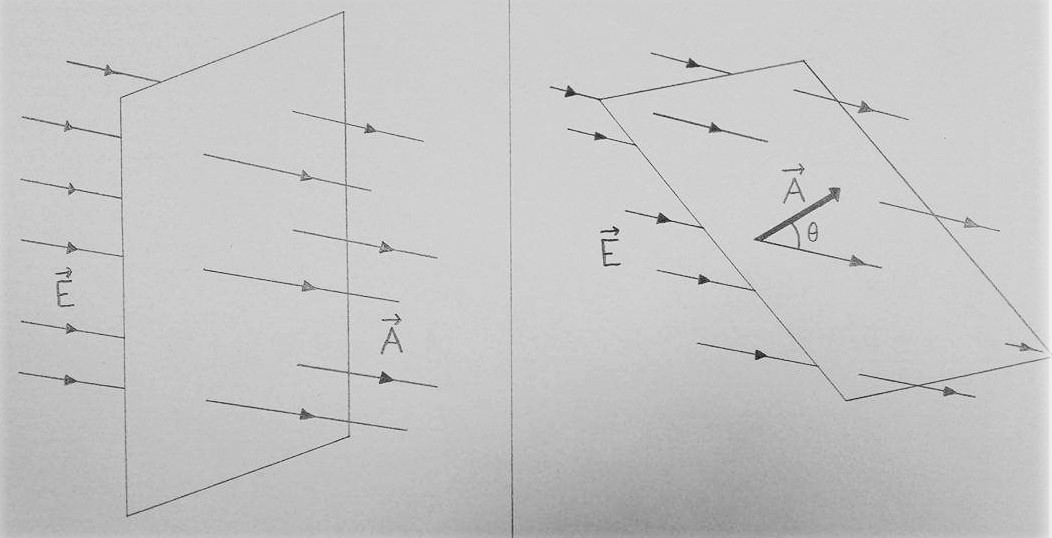
\includegraphics[scale=0.5]{Vildledning/Schematics/vinkelflux.jpg}
\caption{Figur Vinkelflux}
\end{figure}

Gauss's lov angiver ikke kun den elektriske flux, men den kan benyttes til at beregne den flux, der forløber over et bestemt areal. Derved skal der integreres i forhold til overfladen, samt at vektor A skal ganges med en faktor d, altså det bliver $\Phi = \int \vec{E} \bullet d \vec{A}$, som igen kan skrives som $\Phi = \int E \cdot dA \cdot cos(\theta)$. Herefter tager Gauss relation til det cirkulære felt omkring en positiv ladning. A bliver i denne sammenhæng formlen for en kugles overflade $4 \pi r^2$, mens integralet ophæves, da der nu er tale om hele overfladen igen. Herfra er det: $\Phi = E \cdot 4 \pi r^2$

Det elektriske felt E er også angivet til at være $\frac{kq}{r^2}$. Ud fra dette fås den elektriske flux til: $\Phi = \frac{kq}{r^2} \cdot 4 \pi r^2 = 4 \pi k q$. k er derudover defineret som $\frac{1}{4 \pi \epsilon_0}$, hvilket indsættes i forrige formel, altså: $\frac{4 \pi q}{4 \pi \epsilon_0} = \frac{q}{\epsilon_0}$.

q angiver den omkransede ladning for en lukket overflade. Derved bliver Gauss's lov til følgende:

\centerline{$\oint \vec{E} \bullet d \vec{A} = \frac{q}{\epsilon_0}$}

\begin{itemize}
\item Elektromagnetisme
\begin{itemize}
\item Ampère's lov
\end{itemize}
\end{itemize}
Ampère's lov beskriver relationen mellem magnetiske feltstyrker og størrelsen af en jævn strøm gennem en ledning givet over længden l. Ampère tager udgangspunkt i ledningens center og følger magnetfeltet, som omkredser ledningen. Her er magnetfeltets styrke defineret ved vektoren $\vec{B}$, og et definerede linjestykke af magnetfeltets længde angives som $\vec{dl}$. For at beregne den jævne strøm gennem ledningen, skal der tages integralet af de to vektorer prikket sammen. Herved beskrives Ampére's lov:

\centerline{$\oint \vec{B} \bullet \vec{dl} = \mu_0 I$}

Vektor $\vec{B}$ er angivet ved $\frac{\mu_0 I}{2 \pi r}$, da der arbejdes med et cirkelformet magnetfelt. Derudover er det lukkede integral af $\vec{dl}$ den totale længde af cirkelperiferien angivet ved $2 \pi r$. Produktet mellem disse vil dermed blive $\mu_0 I$, som findes på højre side af Ampére's lov.


\begin{itemize}
\item Faraday's lov
\end{itemize}
En af de begreber, som elektromagnetisme beskriver, er induktion af spænding ved hjælp af magnetisme. Magnetisk flux ligner til delt elektrisk flux, som beskrevet tidligere. Dette giver integralet over det magnetiske felt prikket med et bestemt overfladeareal: $\Phi_B = \int \vec{B} \bullet \vec{dA}$

En induseret strøm opstår ikke fra den magnetiske flux alene, men ved en ændring i den magnetiske flux. Dette betyder, at der bliver induceret spænding, hvis der sker en ændring af magnetfeltets styrke, den påvirkede overflades størrelse eller vinklen for, hvordan det magnetiske felt går gennem den pågældende overflade.

Faraday benytter den magnetiske flux til at beskrive den inducerede spænding ved:

\centerline{$\varepsilon = -1 \cdot \frac{d \Phi_B}{dt}$}

Ændringen af den magnetiske flux optræder ofte modsat af den inducerede spænding, så derfor ganger Faraday en faktor -1 på det differentierede udtryk af den magnetiske flux. Den magnetiske flux kan også beskrives som $\vec{B} \bullet \vec{A}$ eller $B \cdot A \cdot cos(\theta)$.
\begin{itemize}
\item Maxwell's ligninger (Forbindelse mellem Faraday og Ampère)
\end{itemize}
Ved trådløs opladning arbejdes der med at omdanne elektrisk flux til magnetisk flux gennem spolen ved transmitteren, hvorefter den magnetiske flux igen skal omdannes til en elektrisk flux ved modtageren. For at beskrive hvordan elektriske felter omdannes til magnetisk flux, ses der på Ampére's lov. Herefter kan overgangen fra magnetfelt til elektrisk flux beskrives gennem Faraday's lov. Derefter kan der ses på Maxwell's ligninger, som bygger videre på Ampère's og Faraday's love, hvorved der kan skabes en sammenhæng.

Maxwell indså, at der måtte foretages modifikationer for Ampére's lov, hvis der skulle kunne skabes symmetri med Faraday's lov. Ved Maxwell's ligninger er Faraday's lov opgivet som det lukkede linjeintegrale af det magnetiske felt, som er lig det negative differentiale af den magnetiske flux i forhold til tid: $\oint \vec{E} \bullet \vec{dl} = -1 \cdot \frac{d \Phi_B}{dt}$.

Herefter kan der tages et blik på Maxwell's modificerede udgave af Ampère's lov. Maxwell har her udbygget formlen, så der skabes en symmetri med Faraday's lov. Derved bliver Ampère's lov omskrevet til, at det lukkede linjeintegrale af det magnetiske felt er lig den elektriske spænding lagt sammen med differentialet af den elektriske flux i forhold til tiden, hvorpå der er ganget en faktor bestående af produktet mellem permeabilitetskonstanten og permittivitetskonstanten: $\oint \vec{B} \bullet \vec{dl} = \mu_0 \cdot I + \mu_0 \epsilon_0 \cdot \frac{d \Phi_E}{dt}$.

Grunden til, at Maxwell udbygger Ampère's lov, er, at loven kun er gældende for, at en stabil strøm er med til at danne en magnetisk flux. For at skabe symmetri med Faraday, udformede Maxwell sin teori om, at elektrisk flux også er gældende for at danne magnetisk flux ved en ustabil strøm. Derved er udtrykket $\mu_0 \epsilon_0 \cdot \frac{d \Phi_E}{dt}$ tilføjet til det oprindelige udtryk.

\textcolor{red}{DETTE ER GAMMEL FYSIK}

\newpage